\documentclass{article}
\title{MyPlate Project}
\author{Henry Oehlrich}
\date{08-31-2023}

\usepackage[margin=1.5in]{geometry}
\usepackage{graphicx}
\usepackage{caption}
\usepackage{subcaption}
\usepackage{sectsty}
\graphicspath{{~/Documents/notebook/school/science/health/images/}}

\sectionfont{\fontsize{12}{15}\selectfont}

\begin{document}
\maketitle{}
\section{Why did you choose this meal and how does this meal reflect your
family’s health needs?}

I chose this meal because it can be cooked entirely outside of the kitchen,
limiting the amount of cleanup required. My family tends to eat a lot of
chicken and also strays away from dairy products.

\section{Was your meal proportionate to the guidelines of MyPlate? If you
excluded a food group such as grains or dairy, justify this decision based on
your family’s health needs.}

My meal is mostly proportionate to the guidelines of MyPlate. My father is
allergic to dairy so I decided to not include any dairy in the meal.

\section{What are the health benefits of eating the foods on the plate? Include
at least two health benefits for at least two foods on the plate.}

The chicken is a good source of protein, while being leaner than red meat. The
vegetables and watermelon are a good source of fiber assisting in digestion.

\section{What was your overall reaction to this project? Did you enjoy it?
Would you have done anything differently upon reflection? Did your family enjoy
it and what was their reaction to the meal and discussion of the meal? Did you
clean the dishes?!}

I enjoyed this project. In retrospect, I would probably choose to smoke the
chickens at a higher temperature for a shorter period of time in order to get
the potatoes crispy without having to transfer them to the grill. My family did
enjoy the meal (it was an amalgamation of different requests from them). I did
do the dishes.

\newpage

\begin{figure}[h]
    \centering
    \begin{subfigure}{.48\textwidth}
        \centering
        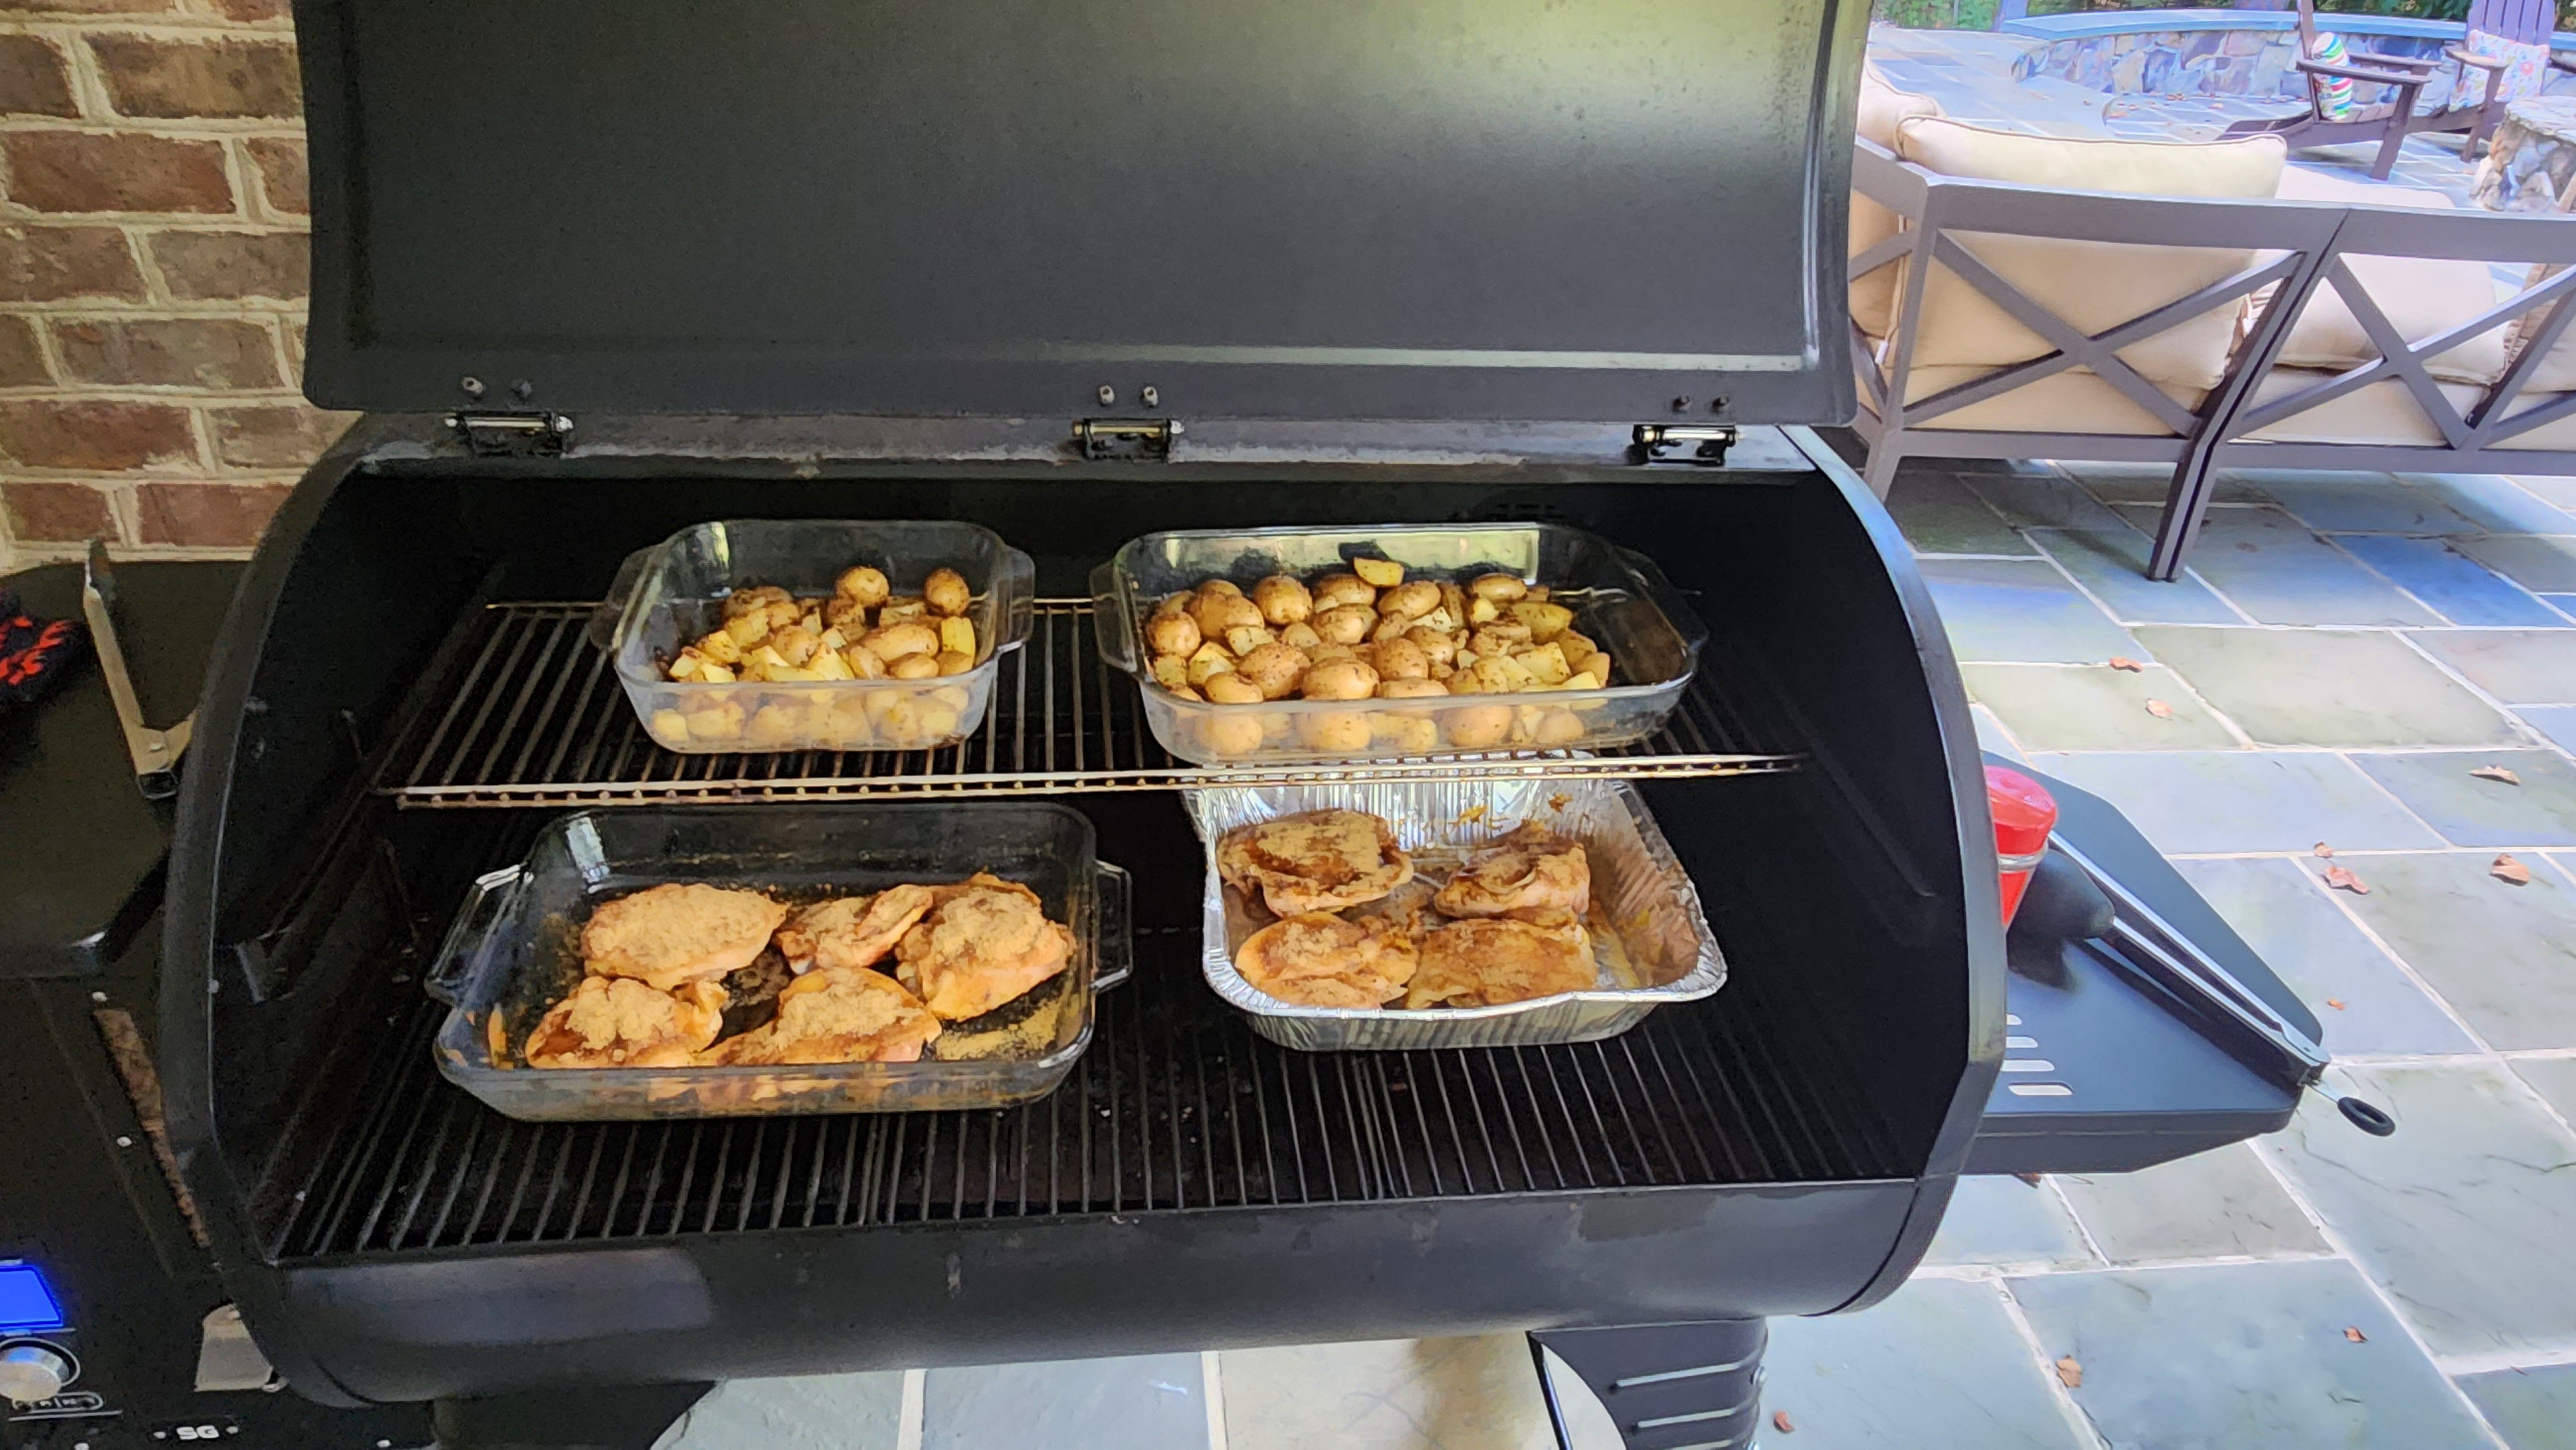
\includegraphics[width=\linewidth]{smoker.jpg}
        \caption{Smoker with chicken and potatoes}
        \label{fig:smoker}
        \vspace{0.1in}
    \end{subfigure}%
    \hspace{\fill}%
    \begin{subfigure}{.48\textwidth}
        \centering
        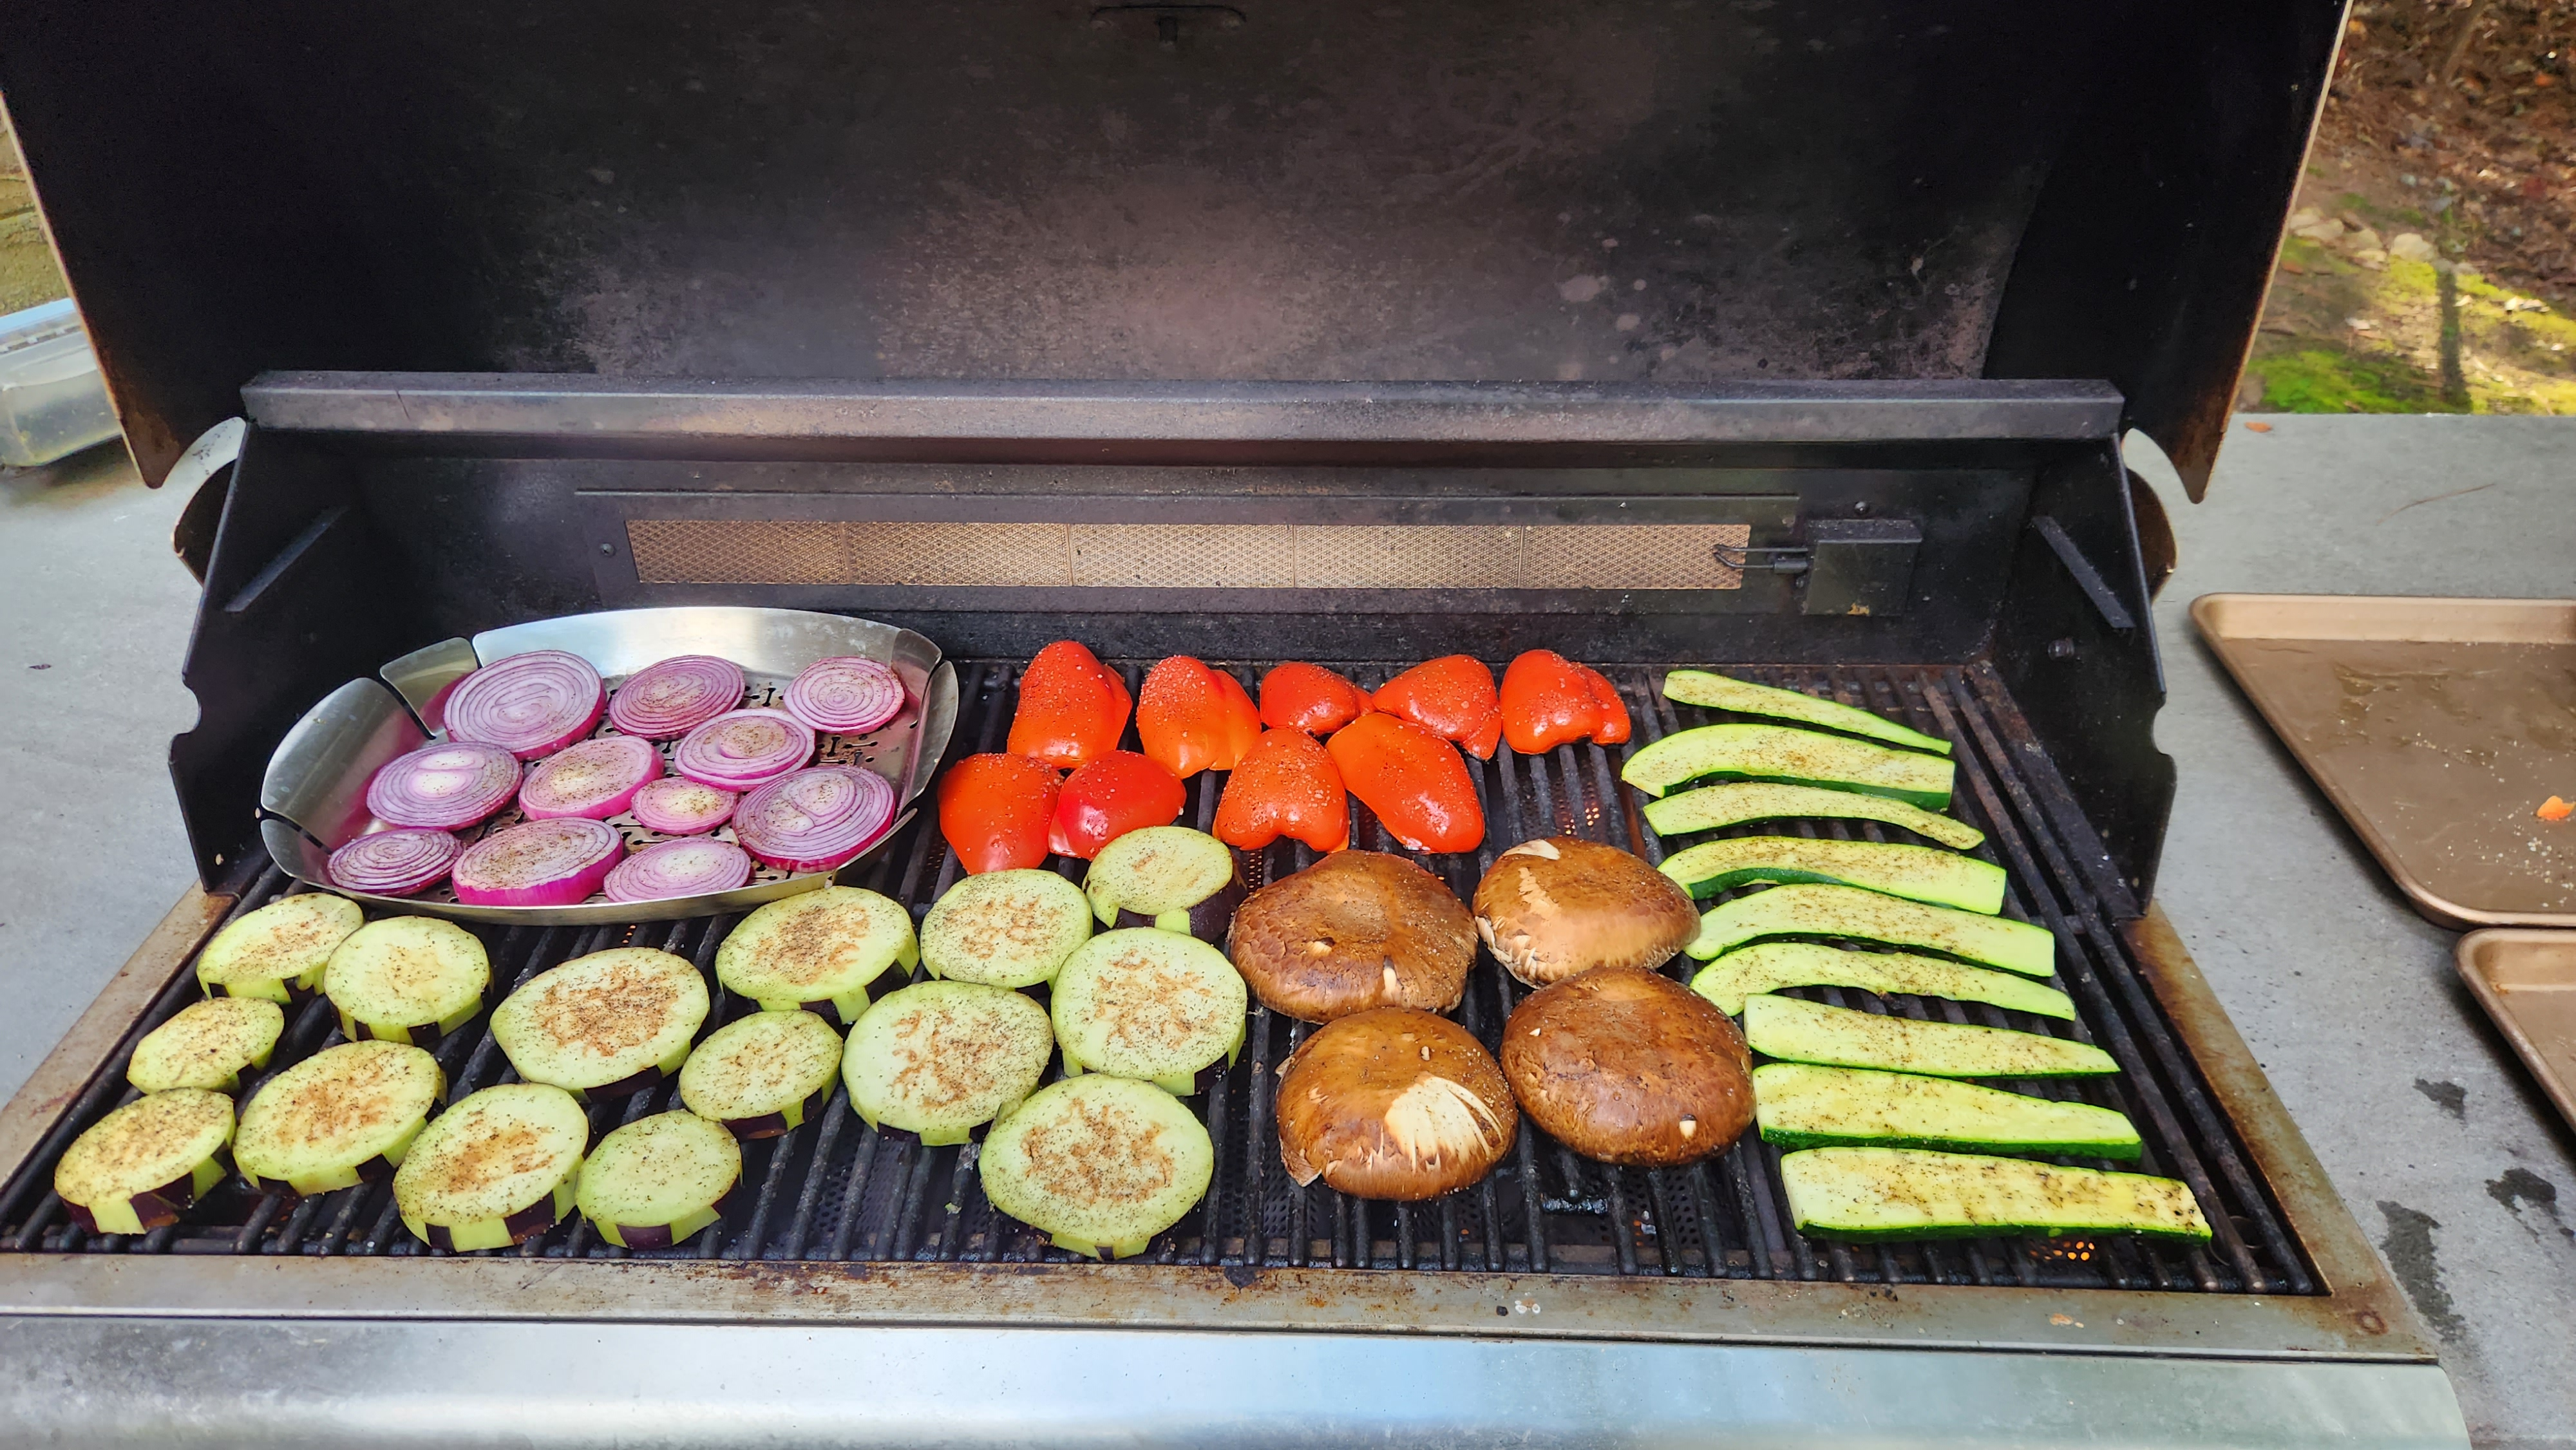
\includegraphics[width=\linewidth]{vegetables.jpg}
        \caption{Grill with vegetables}
        \label{fig:vegetables}
        \vspace{0.1in}
    \end{subfigure}
    \begin{subfigure}{.48\textwidth}
        \centering
        \includegraphics[width=\linewidth]{table.jpg}
        \caption{Table with food}
        \label{fig:table}
    \end{subfigure}%
    \hspace{\fill}%
    \begin{subfigure}{.48\textwidth}
        \centering
        \includegraphics[width=\linewidth]{potatoes.jpg}
        \caption{Smoked potatoes}
        \label{fig:potatoes}
    \end{subfigure}
\end{figure}


\end{document}

